\chapter{DORIS RINEX}
\label{ch:doris-rinex}

\section{Receiver Clock Offsets}

DORIS RINEX contain a ``receiver clock offset'' (\(\tau_{r_offset}\) (as an optional 
field) at the header record of every epoch. E.g. the line
\begin{verbatim}
    ...
    > 2020 01 01 00 00 35.099949800  0  1       -3.248177132 0
    ...
\end{verbatim}
records a receiver clock offset of \SI{35.099949800}{\second} followed by the receiver 
clock offset flag, which in this case is \num{0}. In such record lines, the date (given 
as YYYY MM DD HH MM SS.) is given in the on-board time scale (aka proper time of 
the receiver) and the conversion to the TAI time scale is obtained by adding the 
receiver clock offset.

\textit{Depending on the version of the RINEX file, this offset can have been either 
computed by the DORIS-DIODE navigator, or through a post-fit processing using PANDOR. 
In the first case, the file ends with ``.001'' whereas in the second with ``.010''. 
More information on the computation of (\(\tau_{r-offset}\) are provided in \cite{lemoine-2016}.}

\section{Types of DORIS measurements}
\label{sec:types-of-doris-measurements}

\subsection{Relative Frequency Offset}
\label{ssec:relative-frequency-offset}

DORIS RINEX files (usually) contain a measurement type labeled ``F'' (should be 
recorded in the field \verb|SYS/#/OBS TYPES| at the RINEX header). This measurement 
type is provided for every epoch and is a measure of the relative frequency 
offset of the receiver's oscillator (aka \(\frac{f-f_0}{f_0}\) \num{10e-11}).
Example (rinex header):
\begin{verbatim}
        0.9768        0.0001        0.0011                  CENTER OF MASS: XYZ
D   10  L1  L2  C1  C2  W1  W2   F   P   T   H              SYS / # / OBS TYPES
  2018    01    01    00    00   28.8526816     DOR         TIME OF FIRST OBS
...
                                                            END OF HEADER
> 2018 01 01 00 00 32.589951370  0  3       -3.737269708 0
D01  -2104936.480    -1241282.301   131837622.17412 131837685.14912      -124.650 7
         -114.150 7      5643.911        1025.000 1         6.000 1        85.000 1
D02  -1063469.796    -1862572.573   136575183.93813 136575216.89713      -118.350 7
         -109.250 7      5643.911        1014.000 0       -18.800 0        73.000 0
D03   -826480.354    -2642364.157   148404267.53014 148404098.13114      -115.200 7
         -104.700 7      5643.911         934.000 0       -21.500 0        72.000 0
...                                                            
\end{verbatim}

%\begin{figure}
%\begin{subfigure}{0.45\textwidth}
%  \centering
%  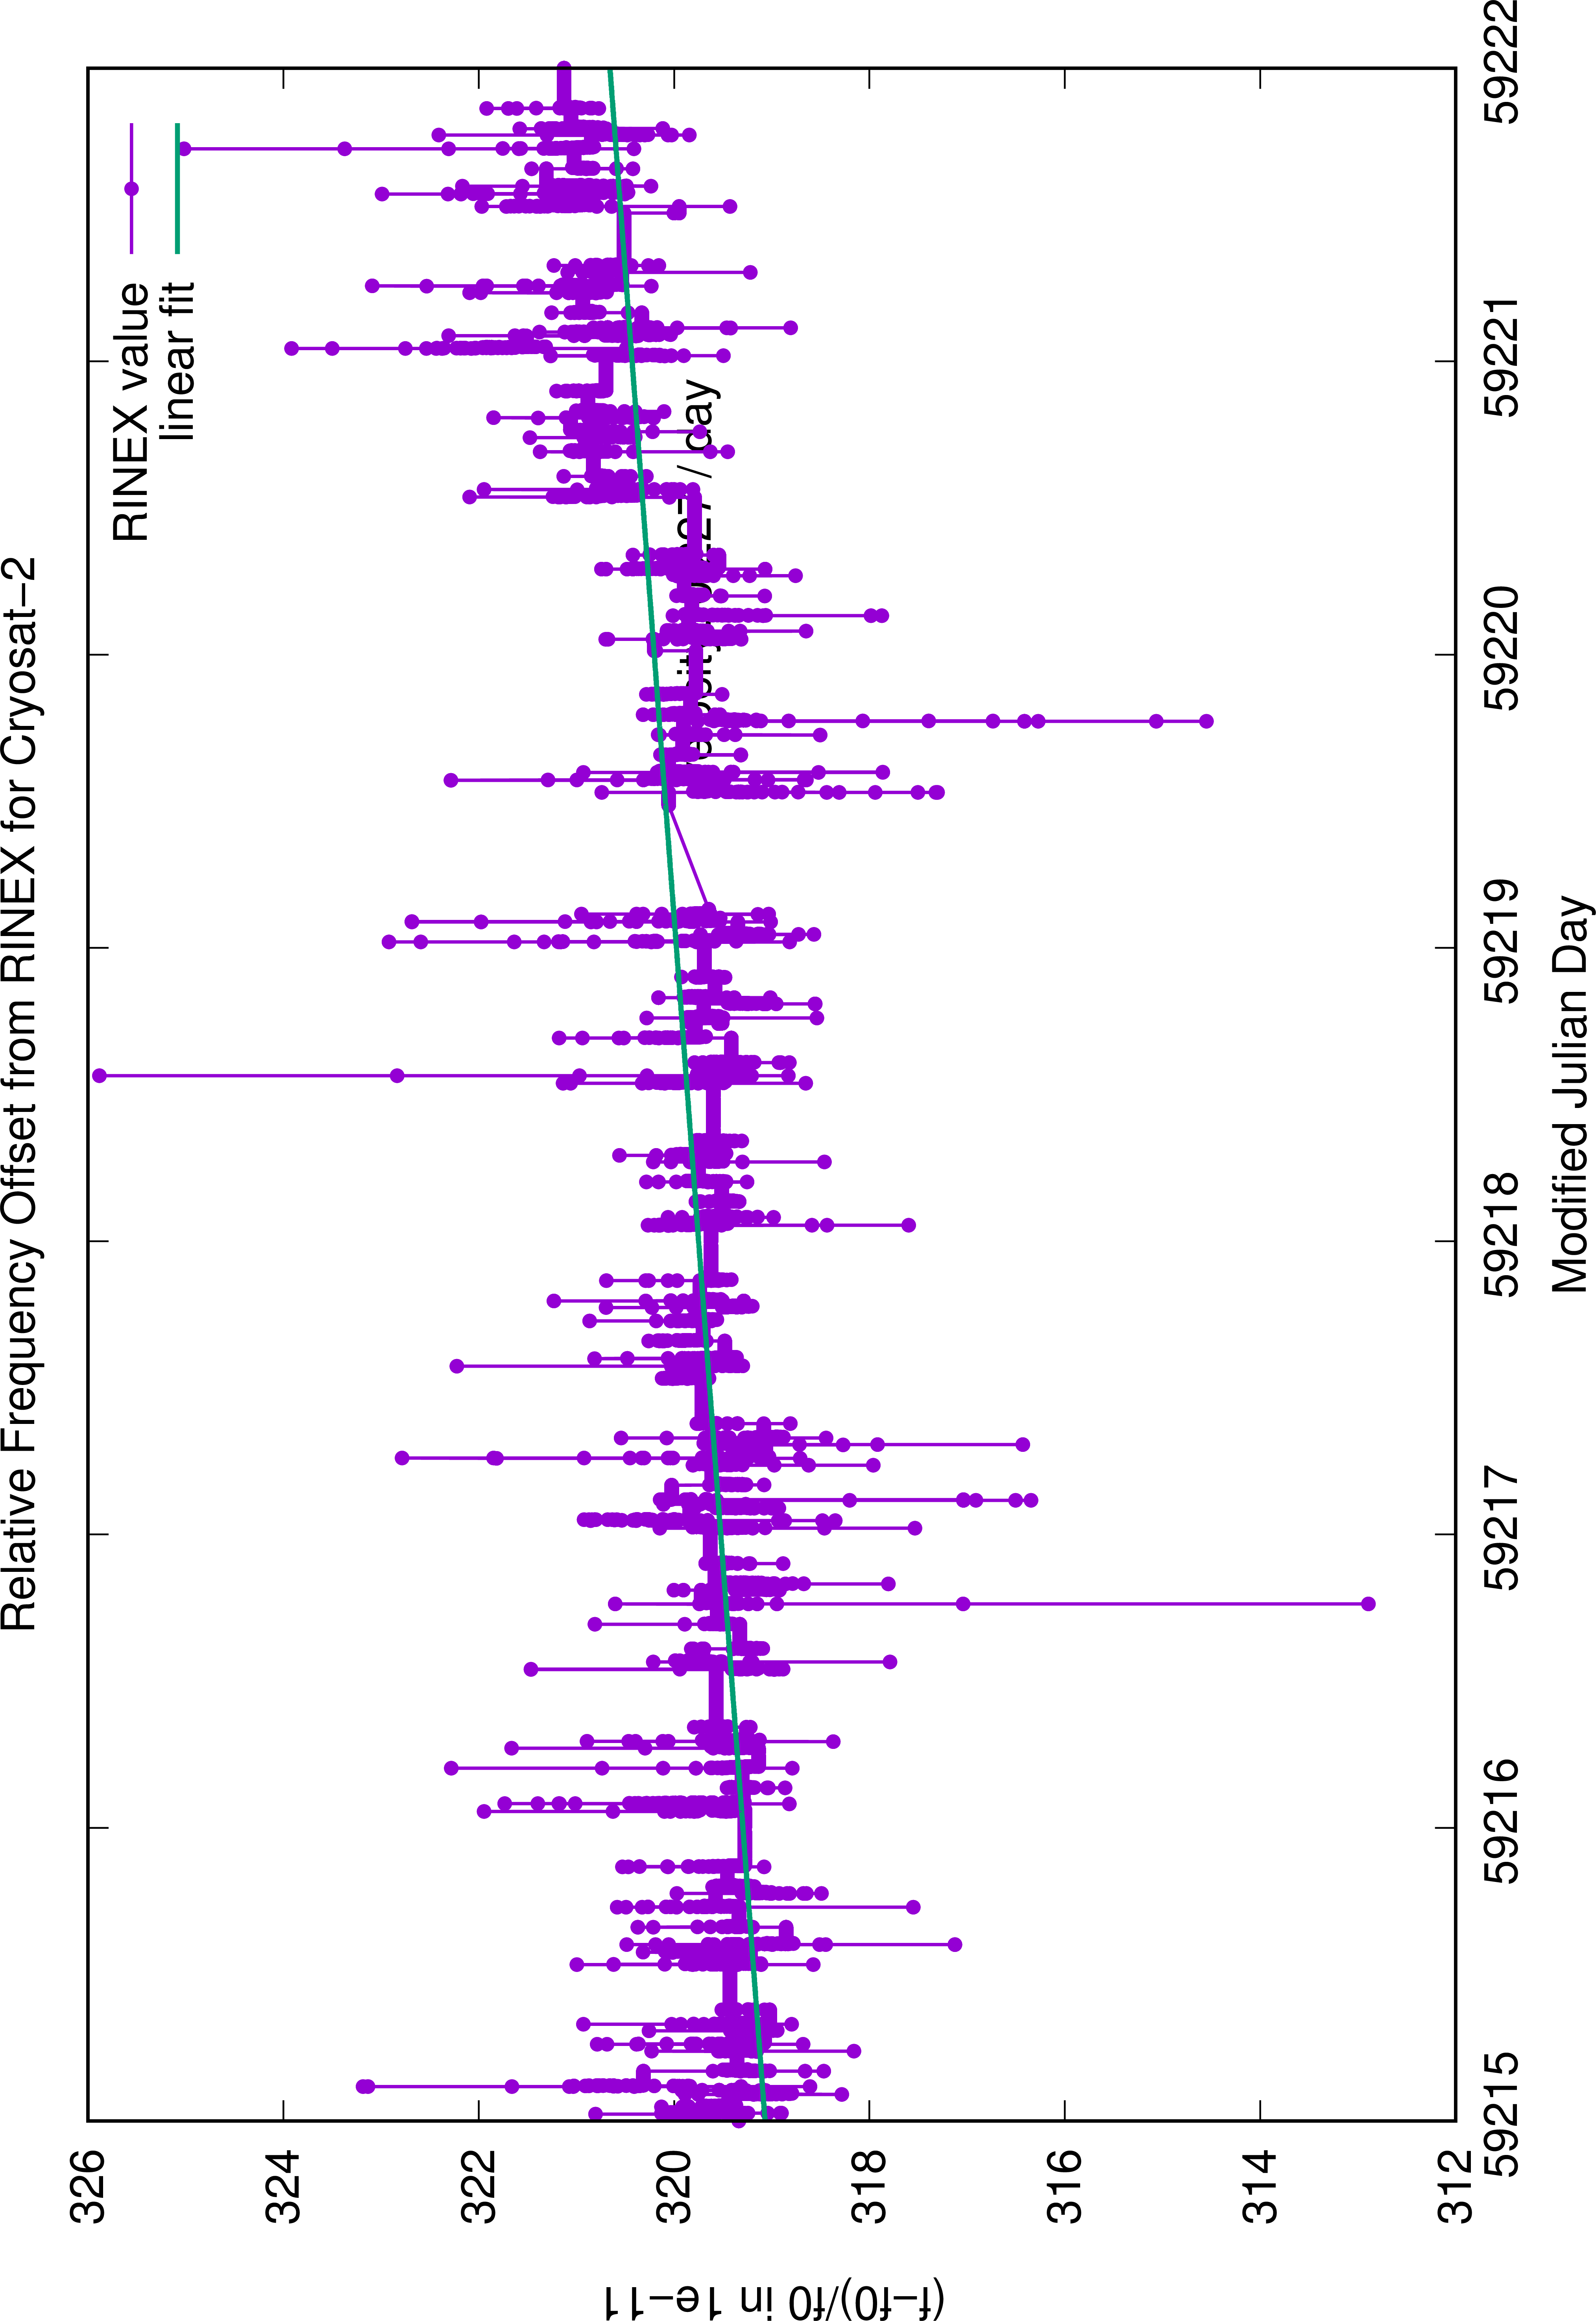
\includegraphics[width=.65\linewidth, angle=-90]{Cryosat-2-RinexRfo}  
%  \caption{\scriptsize RINEX receiver relative frequency offset records for Cryosat}
%  \label{fig:sub-first}
%\end{subfigure}
%\begin{subfigure}{0.45\textwidth}
%  \centering
%  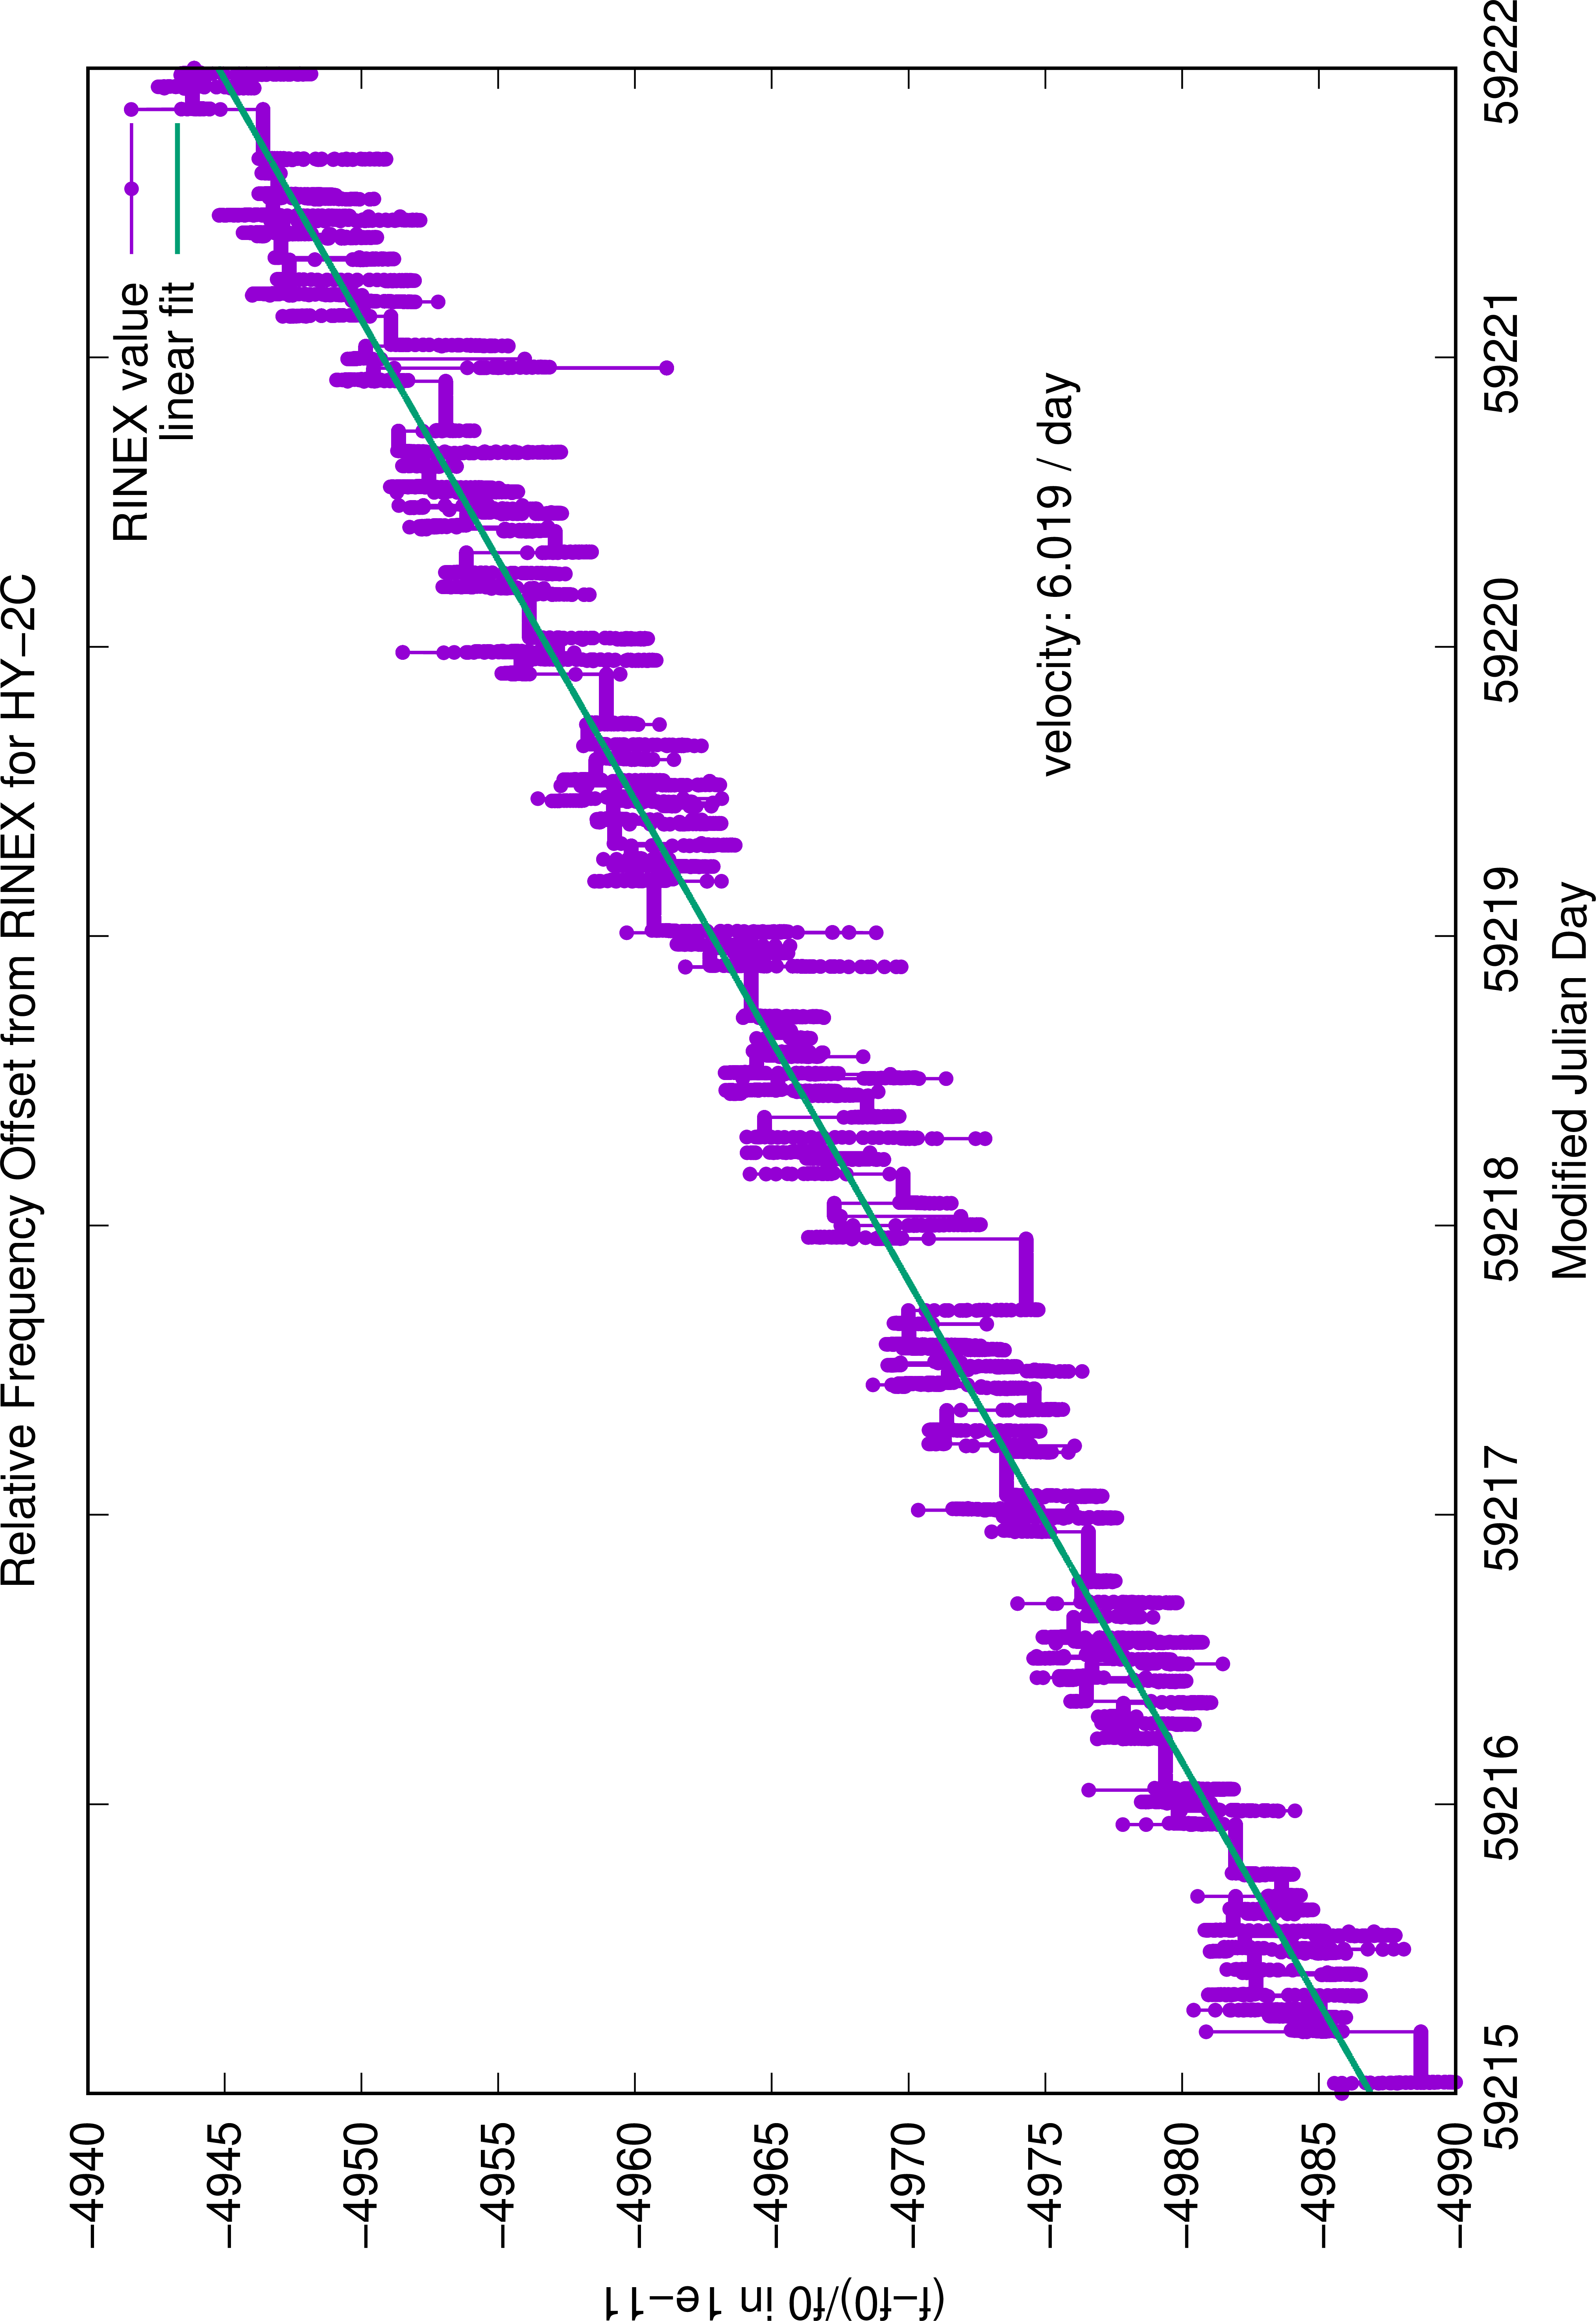
\includegraphics[width=.65\linewidth, angle=-90]{HY-2C-RinexRfo}  
%  \caption{\scriptsize RINEX receiver relative frequency offset records for HY-2C}
%  \label{fig:sub-first}
%\end{subfigure}
%\begin{subfigure}{0.45\textwidth}
%  \centering
%  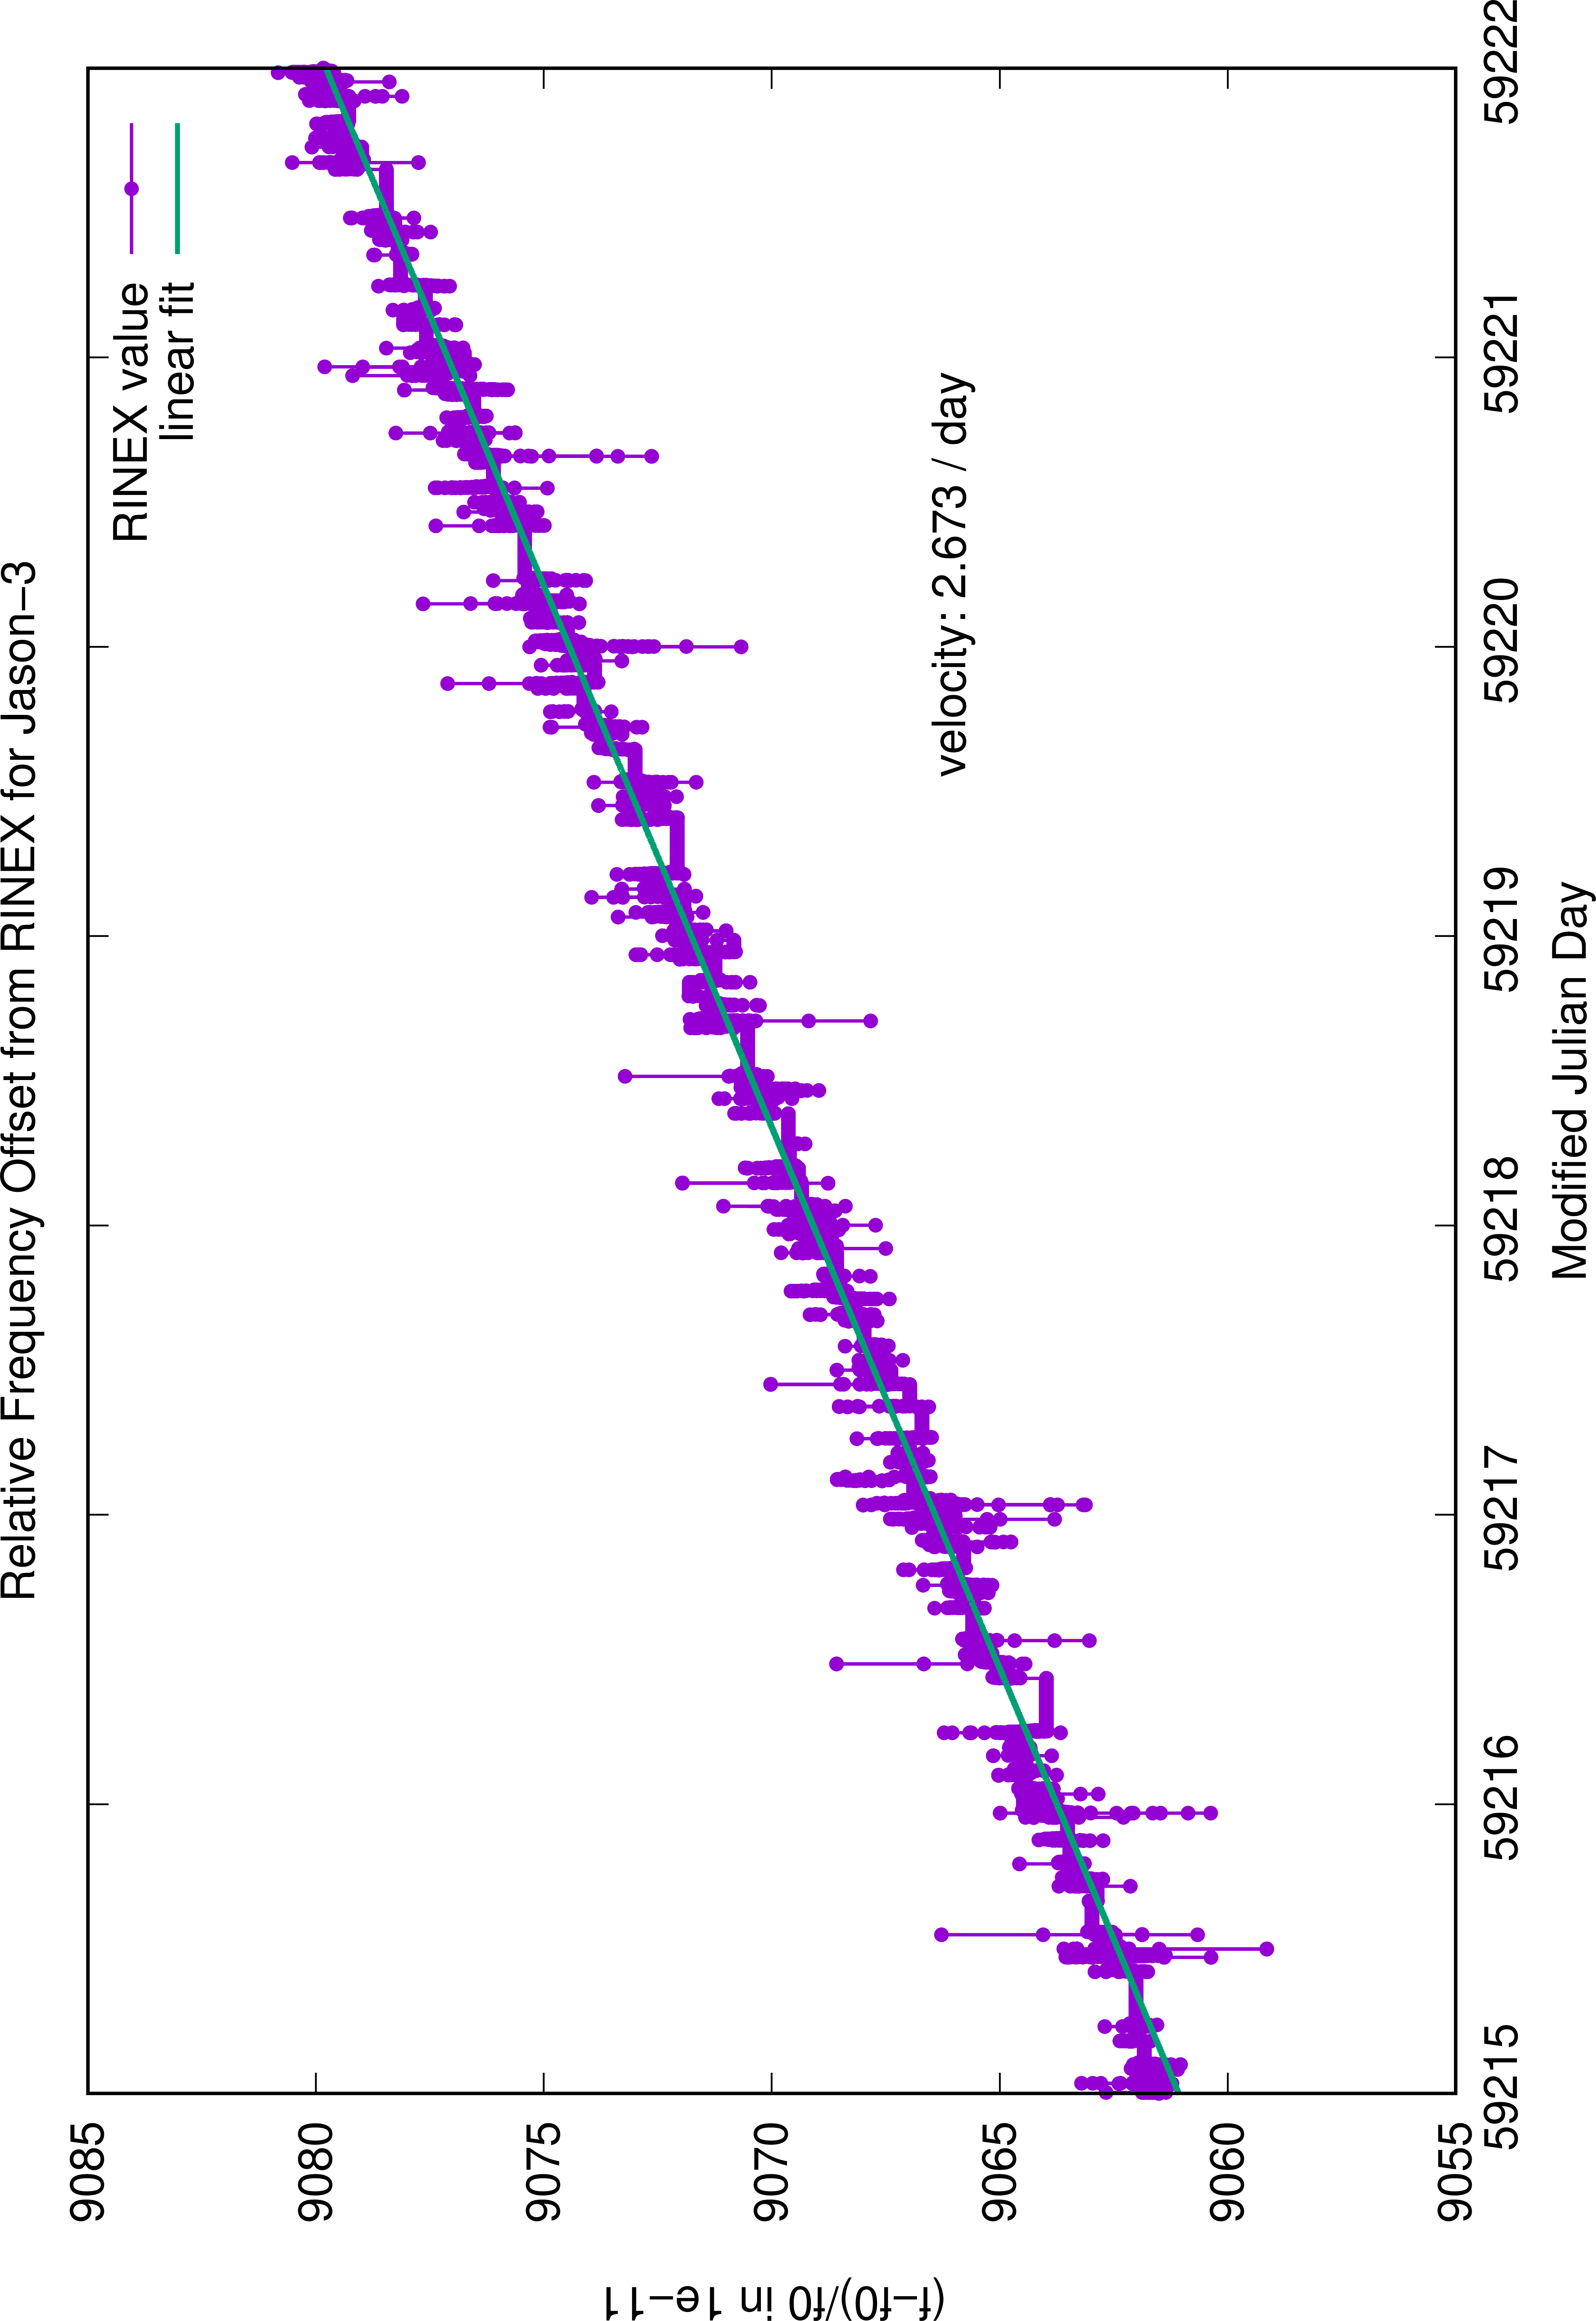
\includegraphics[width=.65\linewidth, angle=-90]{Jason-3-RinexRfo}  
%  \caption{\scriptsize RINEX receiver relative frequency offset records for Jason 3}
%  \label{fig:sub-first}
%\end{subfigure}
%\begin{subfigure}{0.45\textwidth}
%  \centering
%  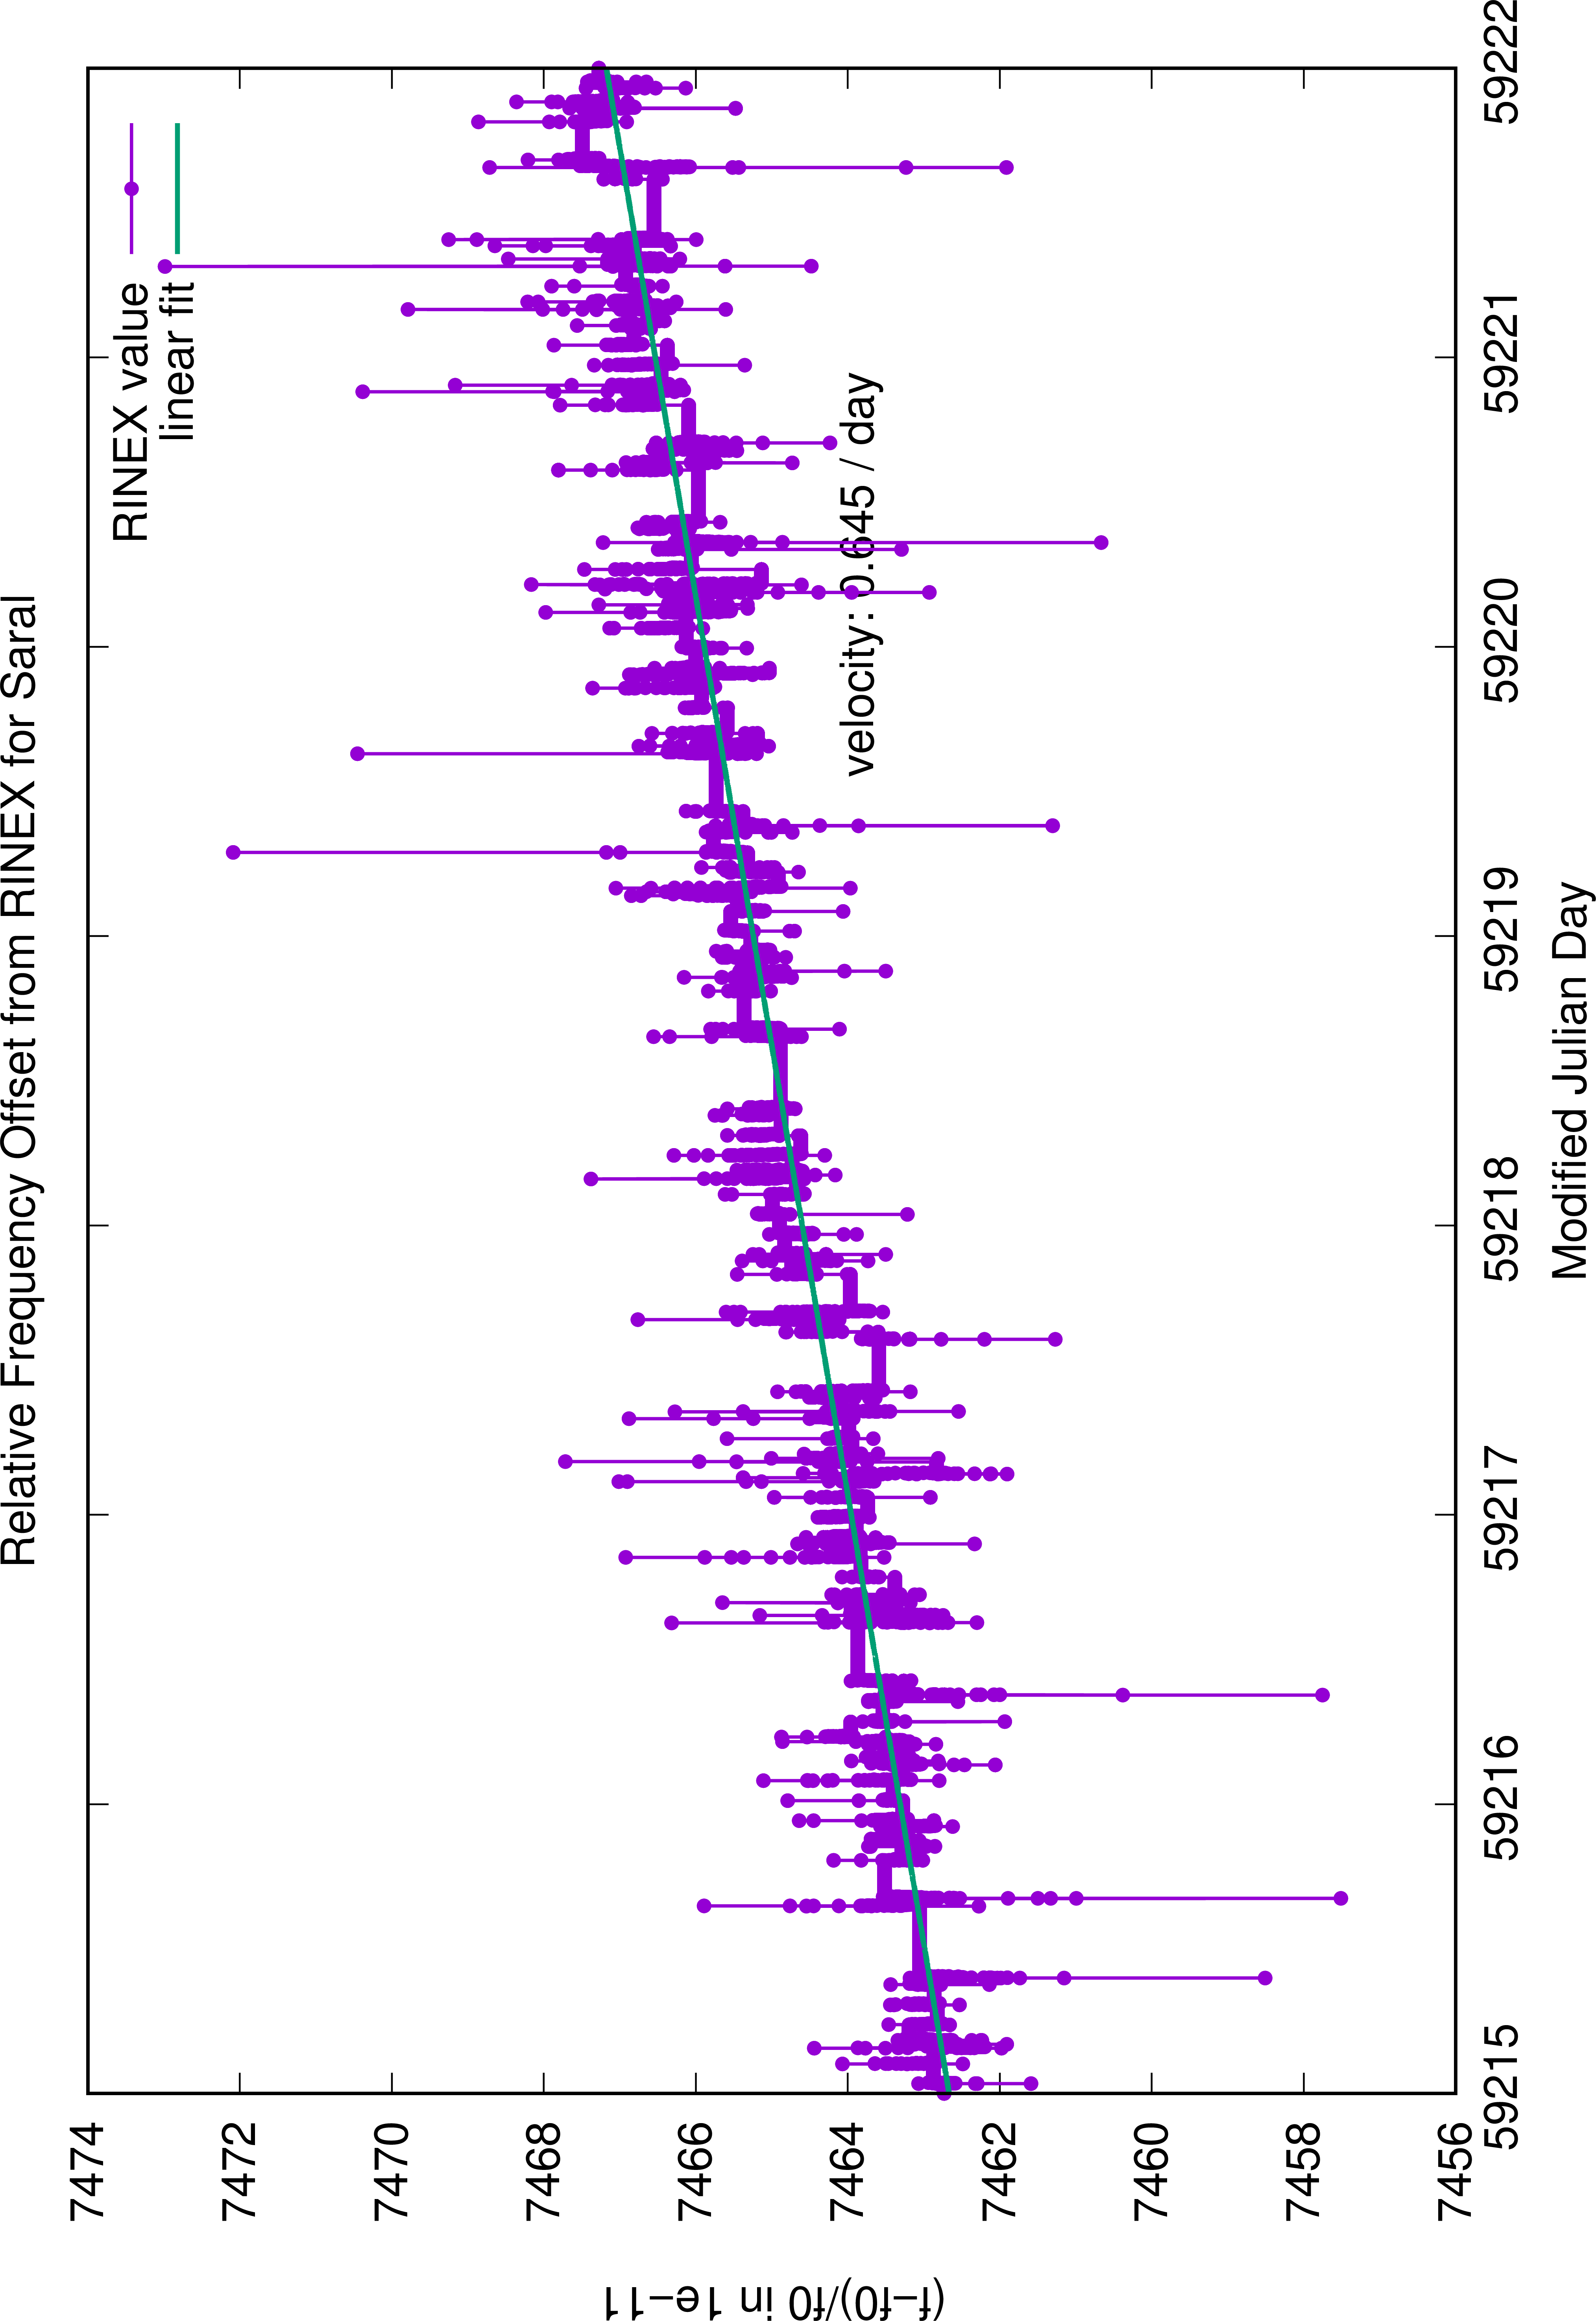
\includegraphics[width=.65\linewidth, angle=-90]{Saral-RinexRfo}  
%  \caption{\scriptsize RINEX receiver relative frequency offset records for Saral}
%  \label{fig:sub-first}
%\end{subfigure}
%\begin{subfigure}{0.45\textwidth}
%  \centering
%  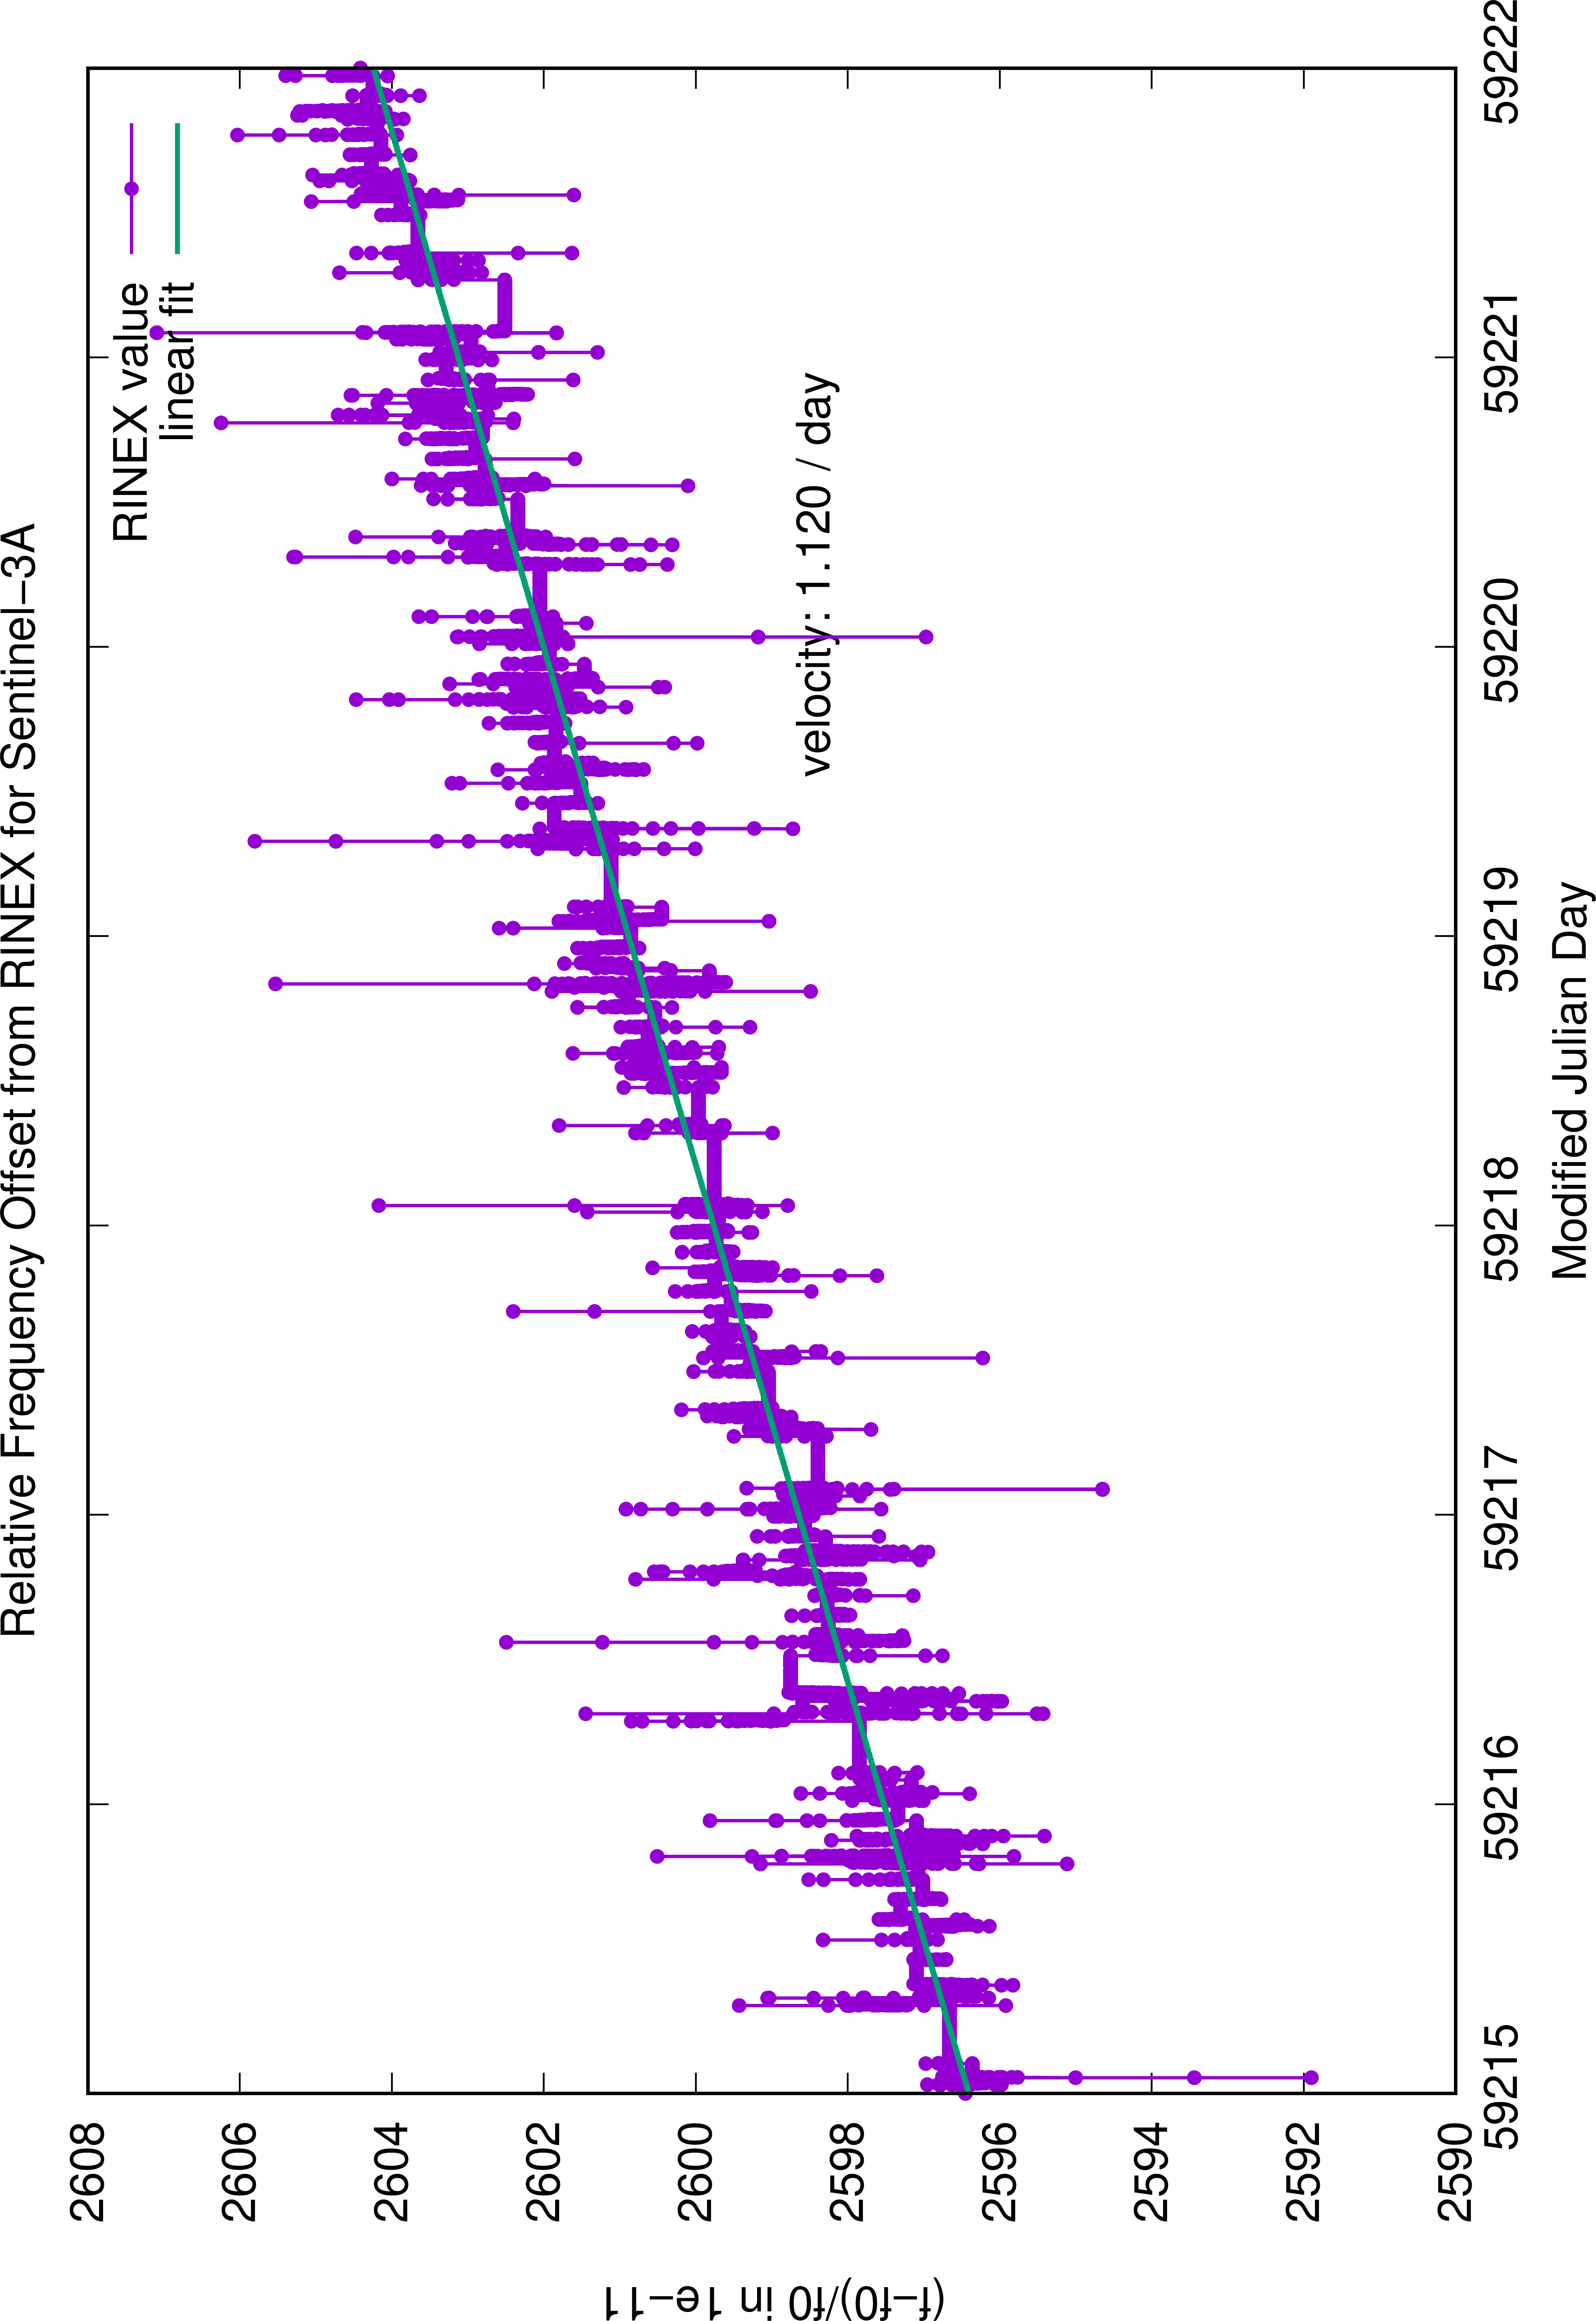
\includegraphics[width=.65\linewidth, angle=-90]{Sentinel-3A-RinexRfo}  
%  \caption{\scriptsize RINEX receiver relative frequency offset records for Sentinel 3A}
%  \label{fig:sub-first}
%\end{subfigure}
%\begin{subfigure}{0.45\textwidth}
%  \centering
%  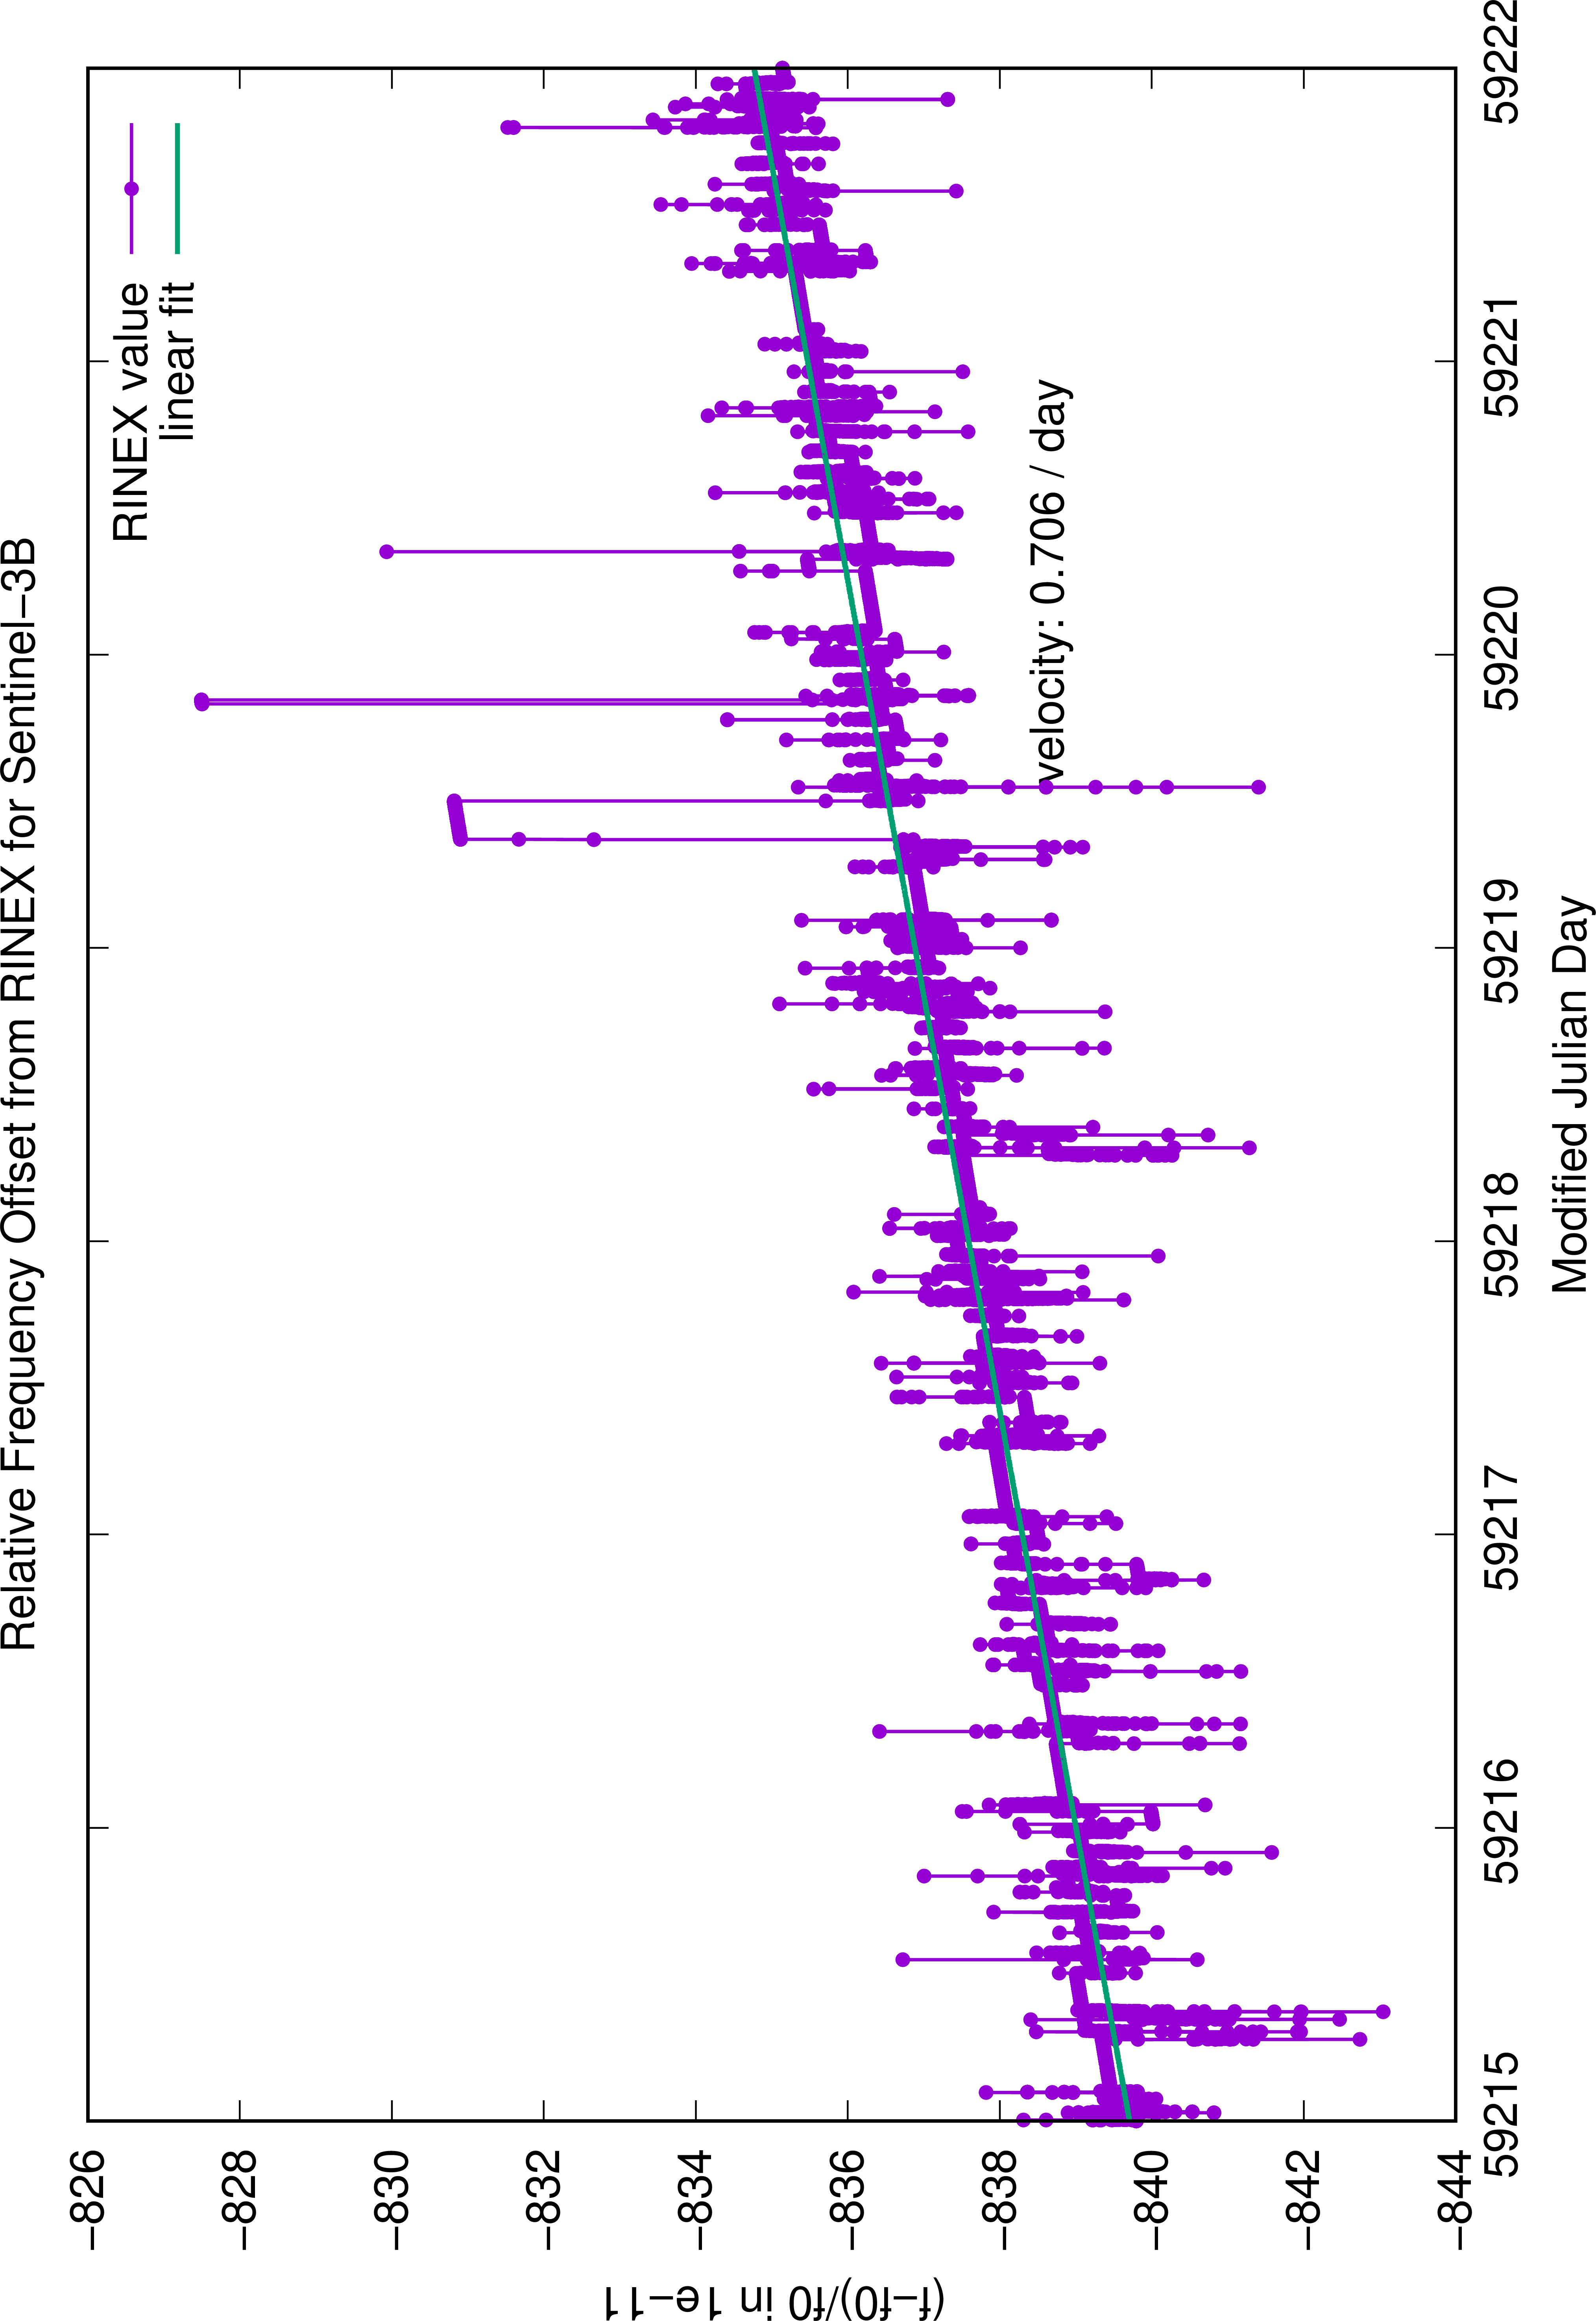
\includegraphics[width=.65\linewidth, angle=-90]{Sentinel-3B-RinexRfo}  
%  \caption{\scriptsize RINEX receiver relative frequency offset records for Sentinel 3B}
%  \label{fig:sub-first}
%\end{subfigure}
%\begin{subfigure}{0.45\textwidth}
%  \centering
%  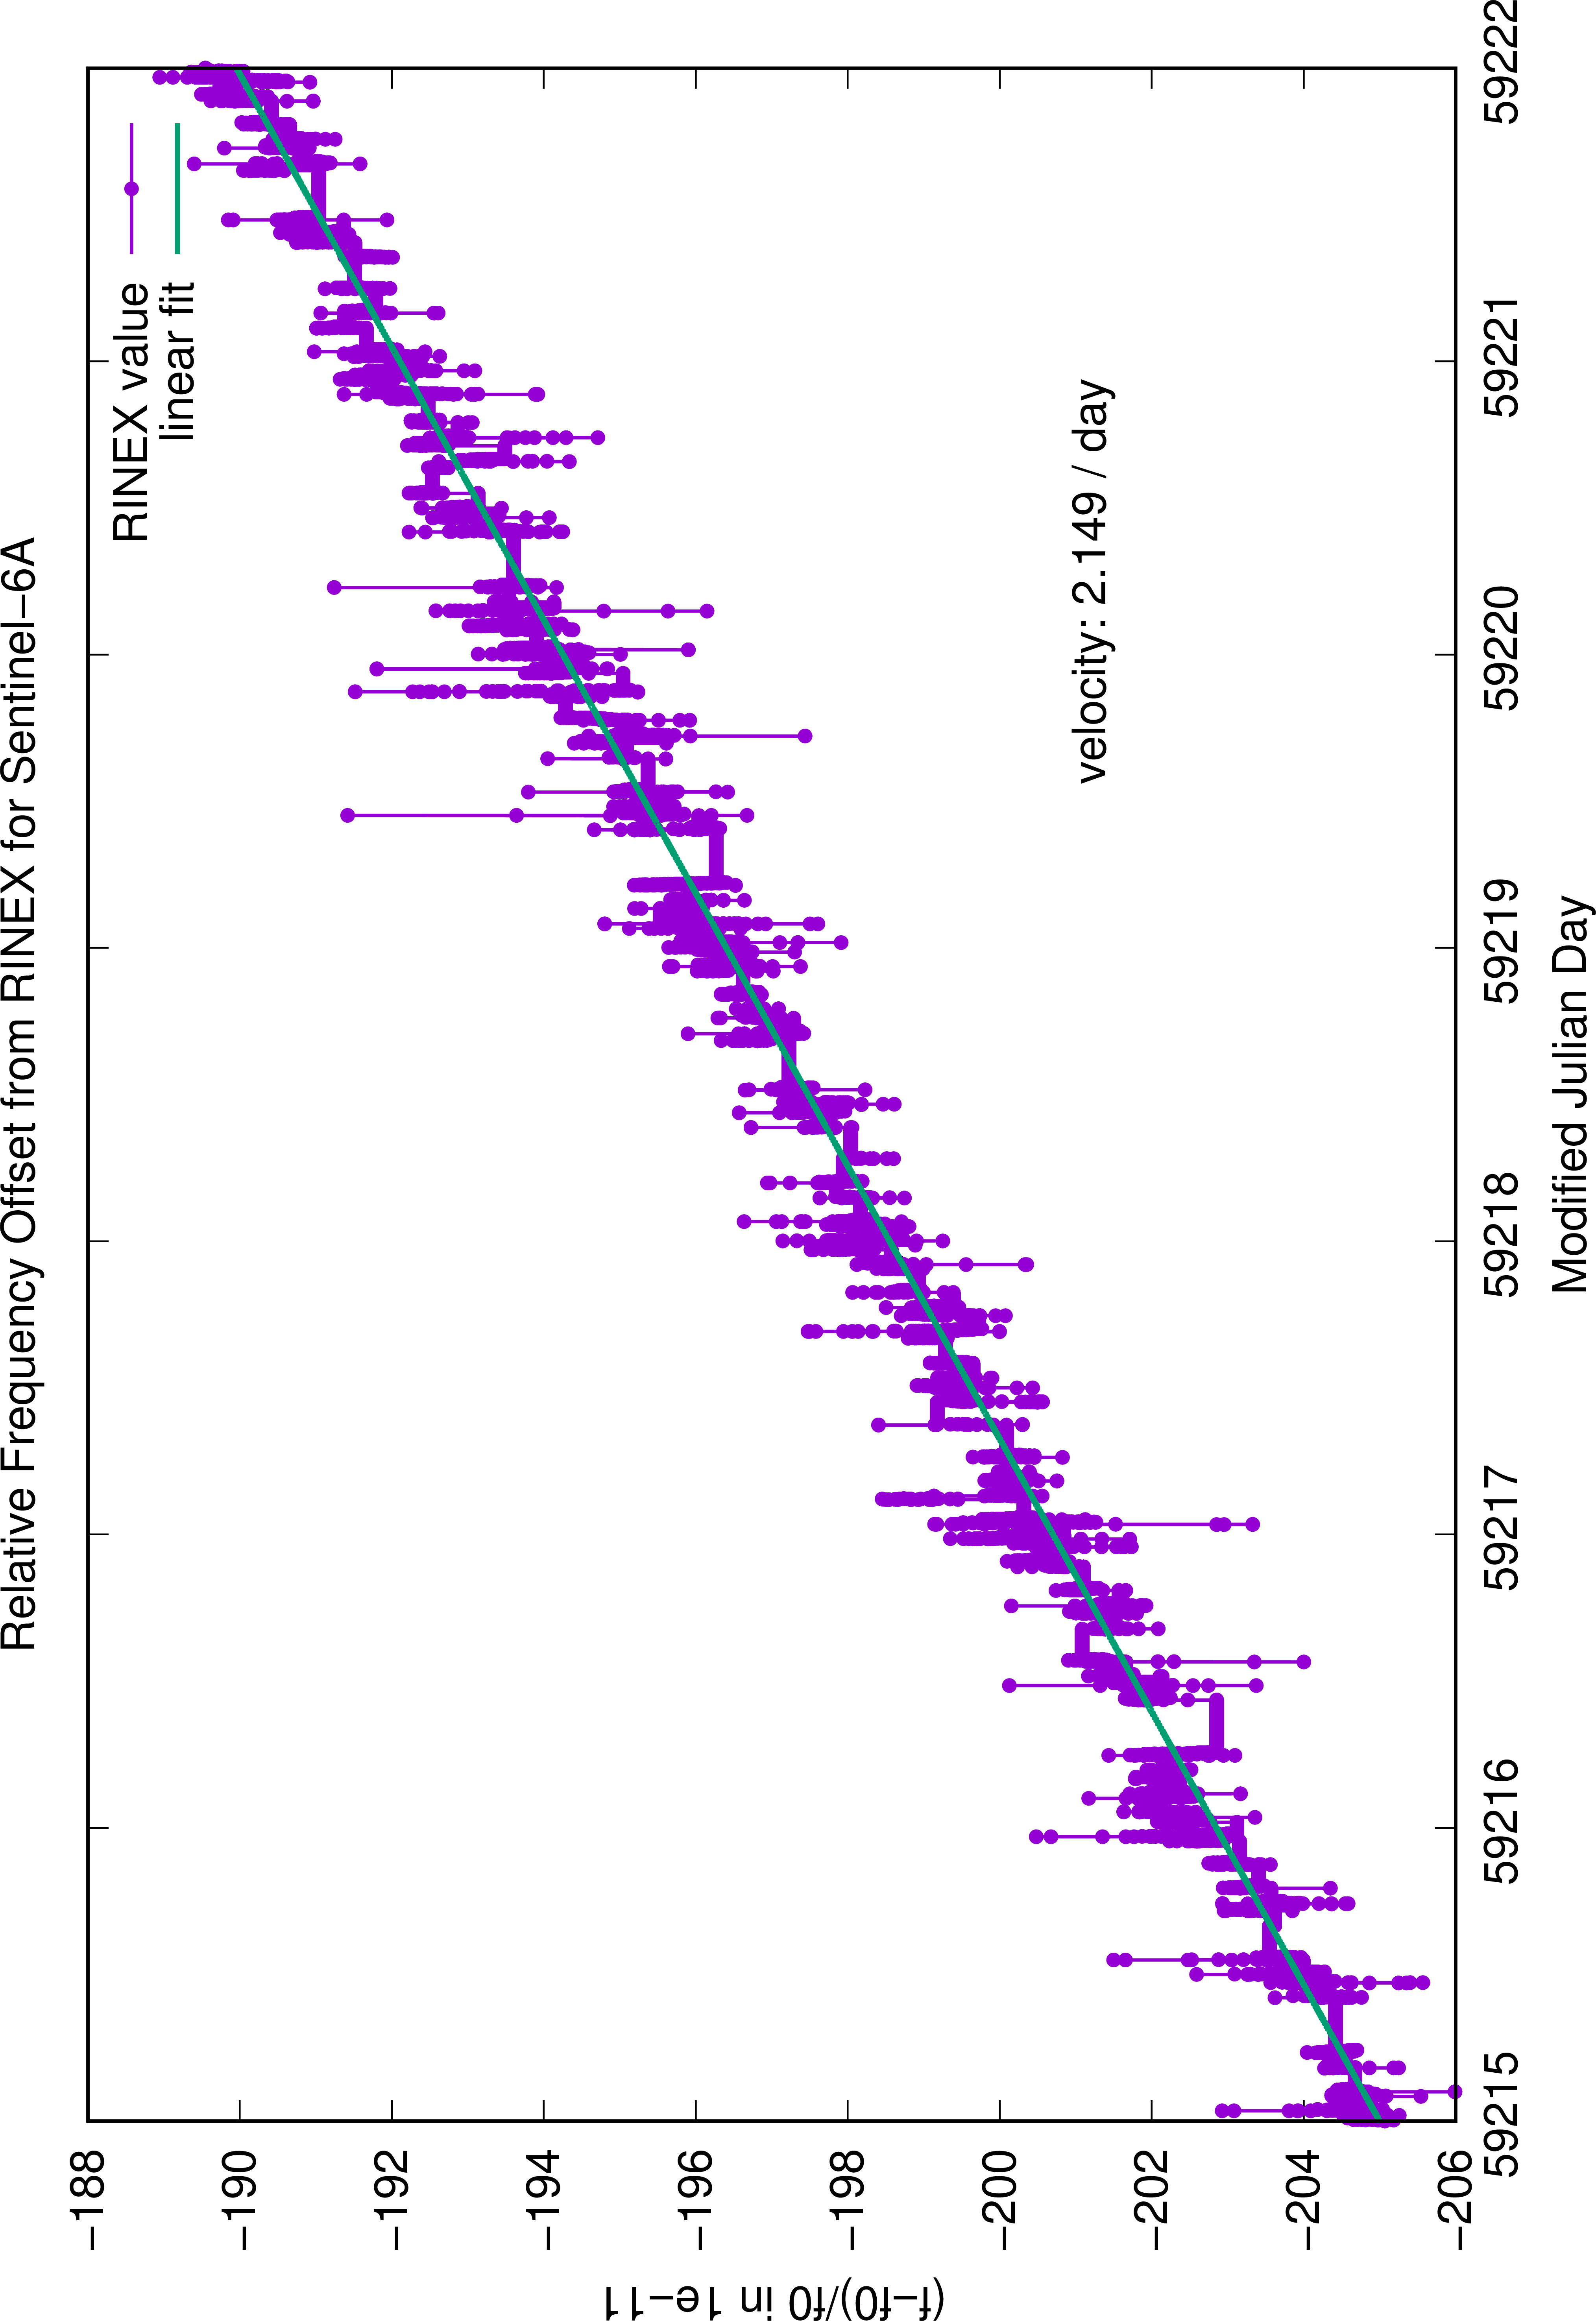
\includegraphics[width=.65\linewidth, angle=-90]{Sentinel-6A-RinexRfo}  
%  \caption{\scriptsize RINEX receiver relative frequency offset records for Sentinel 6A}
%  \label{fig:sub-first}
%\end{subfigure}
%\caption{Receiver relative frequency offset parsed from DORIS RINEX files}
%\label{fig:onw-week-rfo}
%\end{figure}
%